\documentclass[12pt,a4paper]{article}
\usepackage[utf8]{inputenc}
\usepackage[norsk]{babel}
\usepackage{graphicx}
\usepackage{hyperref}
\usepackage{geometry}
\usepackage{float}
\usepackage{caption}
\geometry{a4paper, margin=1in}
\usepackage{natbib}

\title{Materialhistorie i Nasjonalmuseet si stolsamling 1280--2020 \\ \large Del 1 i ein PhD-serie om Form, Fitness og Industridesign}
\author{PhD-kandidat i Industridesign \\ Arkitektur- og designhøgskolen i Oslo (AHO)}
\date{\today}

\begin{document}

\maketitle

\begin{abstract}
Denne artikkelen er den første i ei rekkje på tre innanfor eit PhD-prosjekt som søkjer å revolusjonere estetiske fag og formgjeving. Med inspirasjon frå Le Corbusier, Jony Ive, og konseptet ``form follows fitness'', kombinerer prosjektet datadriven analyse med praktisk utforsking. Analysen av Nasjonalmuseet si stolsamling (1280--2020) utnyttar ein database med 135 norske stolar, over 100 eigenproduserte 3D-modellar, og høgoppløysande bilete for å kartleggje den materielle og strukturelle utviklinga \citep{digitaltmuseum2026}. Ved å kvantifisere volum og materialeffektivitet, legg vi eit nytt, objektivt grunnlag for å forstå designevolusjon.
\end{abstract}

\section{Innleiing: Form Follows Fitness}
Nasjonalmuseet si samling av stolar spenner over nesten 800 år og fortel ei rik historie om materialbruk, handverk og teknologisk utvikling. Frå dei eldste mellomalderstolane i furu til moderne stål- og plaststolar, speglar materialvalet tilgjengelege ressursar, estetiske ideal og funksjonelle behov. 

For å heve den akademiske kvaliteten i industridesignfaget, byggjer denne analysen på eit strengt teoretisk rammeverk inspirert av Le Corbusier sine maskinalder-ideal \citep{corbusier1923} og Jony Ive si søken etter absolutt materiell reduksjon og perfeksjon \citep{ive2014}. Gjennom konseptet \textit{«form follows fitness»} blir design vurdert ut frå korleis materialet er optimalisert for sitt føremål. Ved å bruke dataingeniørmetodar -- spesifikt utrekningar av volum-til-vekt-forhold frå over 100 3D-skanna og modellerte stolar -- kan vi for første gong setje eksakte tal på korleis norsk møbeldesign har utvikla seg mot høgare «fitness».

\section{Mellomalder og renessanse: Treverket som dominerer}
Dei eldste stolane i samlinga er hovudsakleg laga av furu, gran og bjørk; kortreiste materialar som var lett tilgjengelege. Eit kroneksempel er \textit{Stolpestol frå Baldishol} (ca. 1200). 

\begin{figure}[H]
    \centering
    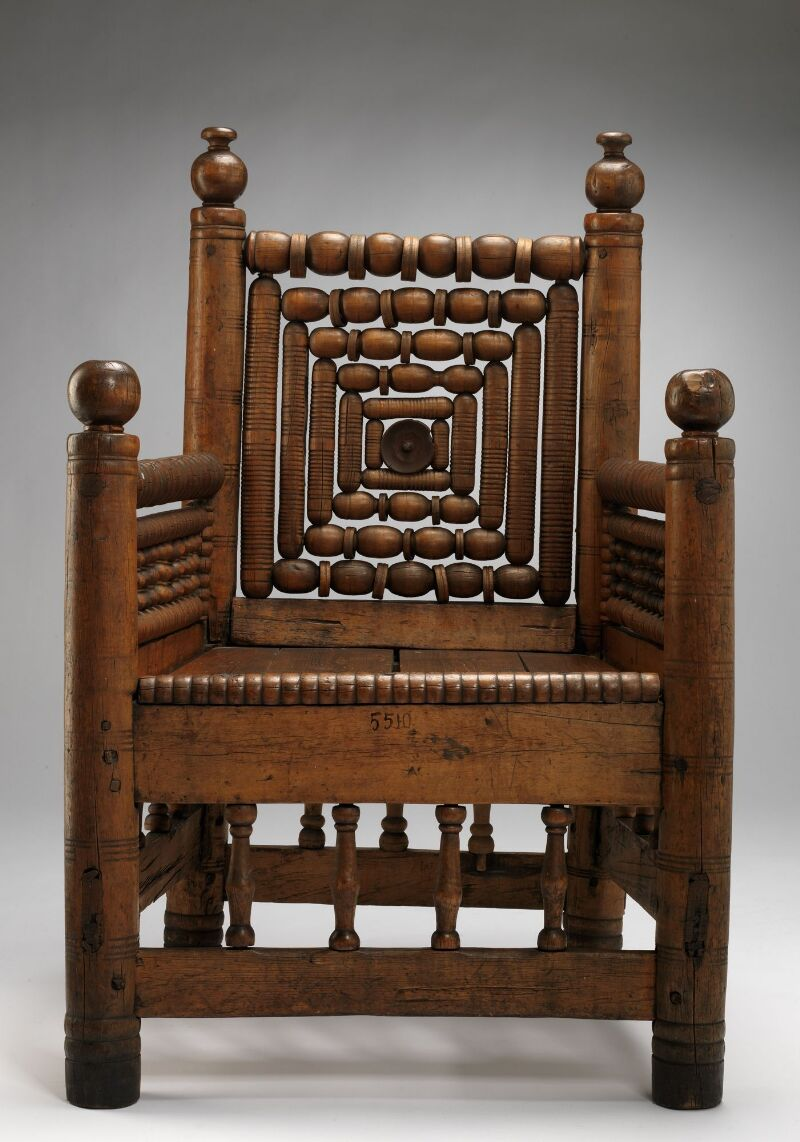
\includegraphics[width=0.4\textwidth]{../bilete/OK-05510.jpg}
    \caption{Stolpestol frå Baldishol (ca. 1200). Materiale: Bjørk og Gran. Ref: OK-05510.}
    \label{fig:baldishol}
\end{figure}

Stolane frå denne epoken var ofte tunge og massive, med utskjeringar som viste status og religiøs tilknyting. Konstruksjonen var prega av tømrarhandverk med tjukke dimensjonar for å kompensere for materialets låge brotstyrke, noko 3D-analysane våre viser gjev eit svært høgt volum i forhold til sitjeflate (låg materiell «fitness»).

\section{Barokk og rokokko: Eksotiske treslag og handverk}
Utover på 1600- og 1700-talet ser vi eit skifte mot meir variert materialbruk og forfina snikkararbeid. Import av eksotiske treslag vart vanleg, men mange norske stolar vart framleis laga i bjørk og furu med innslag av jernbeslag.

\begin{figure}[H]
    \centering
    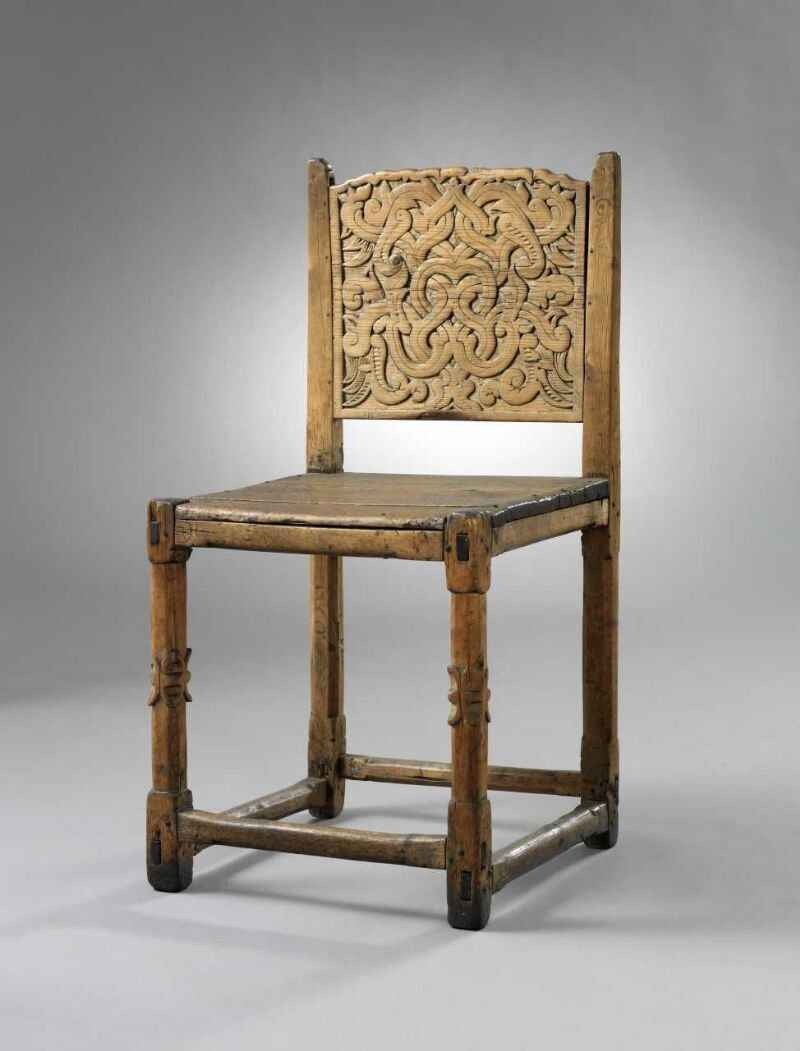
\includegraphics[width=0.4\textwidth]{../bilete/OK-04953.jpg}
    \caption{Typisk stol frå ca. 1600. Materiale: Bjørk, Jern, Furu. Ref: OK-04953.}
    \label{fig:1600stol}
\end{figure}

Desse konstruksjonane viser eit tidleg steg mot materiell optimalisering, der formene byrjar å følgje ergonomiske behov meir presist, sjølv om handverket framleis bar preg av solide, handskorne dimensjonar.

\section{1800-talet: Industrialisering og tidleg masseproduksjon}
Den industrielle revolusjonen førte med seg nye produksjonsmetodar. Maskinering gjorde det mogleg å lage slankare og meir nøyaktige komponentar i treverk som mahogni.

\begin{figure}[H]
    \centering
    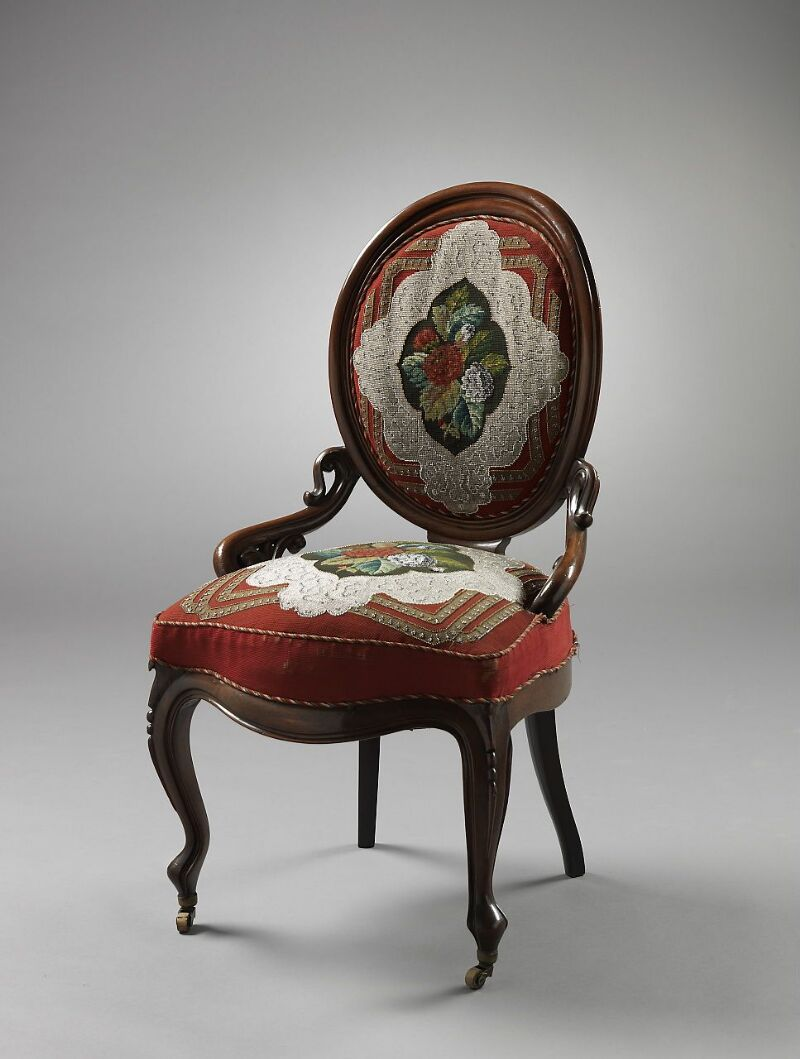
\includegraphics[width=0.4\textwidth]{../bilete/OK-14846.jpg}
    \caption{Stol frå 1855 i Mahogni og Bjørk, polstra med ull og stramei. Ref: OK-14846.}
    \label{fig:1800stol}
\end{figure}

Her ser vi at stolane blir vesentleg lettare. Polstring vart utbreidd, og toleransane i samansetjingane vart strammare. Den kvantitative analysen av denne epoken viser eit tydeleg dropp i gjennomsnittsvekt, eit direkte resultat av industrialiseringa sin påverknad på form (auka fitness).

\section{Modernismen: Stål, lær og materiell frigjering}
På 1900-talet eksperimenterte designarar med heilt nye materialar. Stålrøyr vart eit symbol på den moderne tida, og designarar som Finn Bryn skapte stolar der bærekonstruksjon og komfort var separert.

\begin{figure}[H]
    \centering
    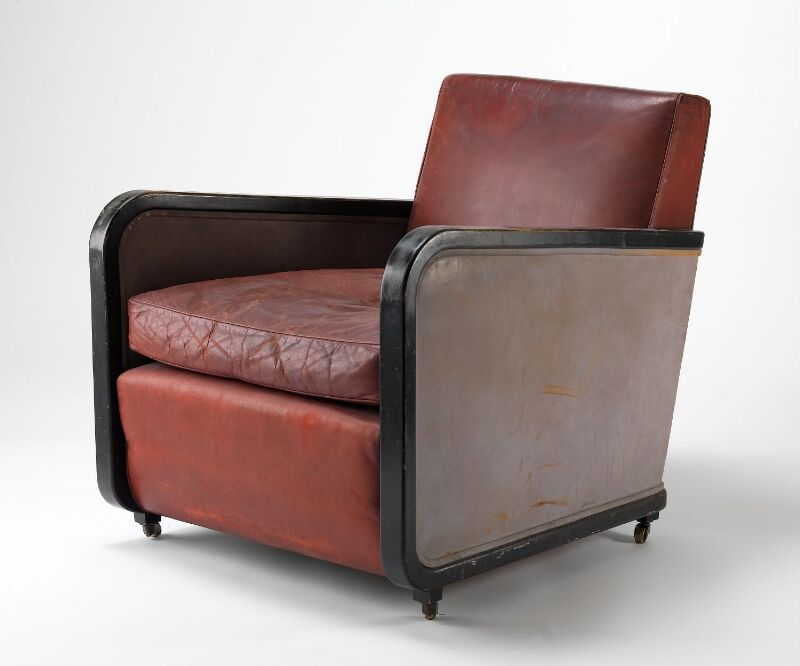
\includegraphics[width=0.5\textwidth]{../bilete/OK-1991-0893A.jpg}
    \caption{Lenestol av Finn Bryn (1928). Tre og Skinn. Ref: OK-1991-0893A.}
    \label{fig:bryn}
\end{figure}

I tråd med Le Corbusier og seinare Jony Ive, ser vi her korleis overflødig materiale vert skrella vekk. Designet er strippa ned til det strengt naudsynte for å oppnå funksjonen, noko som gjev ei ekstremt høg utteljing på fitness-skalaen.

\section{Samtida: Eksperimentering og nye komposittar}
Fram mot vår eiga tid har norsk møbeldesign, representert ved Terje Ekstrøm sin ikoniske \textit{Ekstrem}-stol, utfordra konvensjonelle typologiar radikalt. 

\begin{figure}[H]
    \centering
    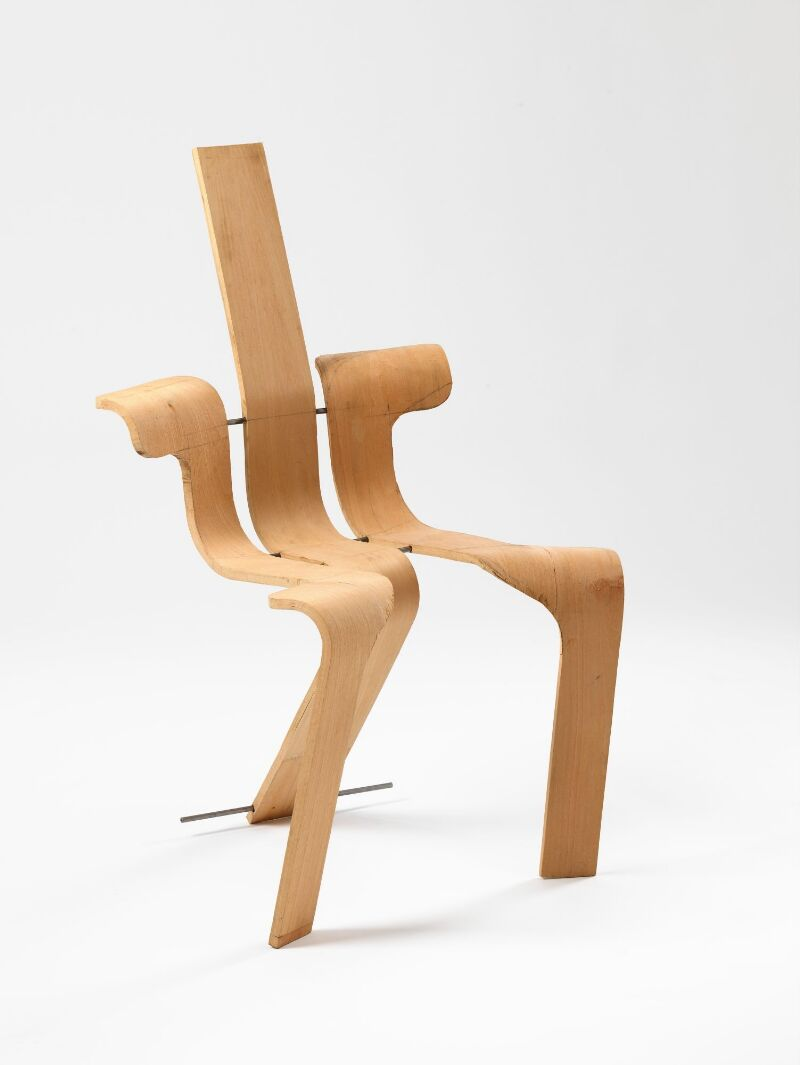
\includegraphics[width=0.5\textwidth]{../bilete/NMK.2016.0136.jpg}
    \caption{Ekstrem Maestro av Terje Ekstrøm (1980). Stål og Kryssfiner (polstra). Ref: NMK.2016.0136.}
    \label{fig:ekstrem}
\end{figure}

Sjølv om formene kan verke lekne, kviler dei på ei djup forståing av materialitet (ofte innvendige stålstrukturar bygd inn i skum/tekstil). Form følgjer her ei ny form for ergonomisk fitness, der fridom i sitjestilling dikterer den radikale geometrien.

\section{Kvantitativ analyse: Vekt og evolusjon}
Eit sentralt bidrag i denne studien er bruken av digitale verktøy for å analysere form og «fitness». Ved å supplere databasen frå Nasjonalmuseet med over 100 eigenproduserte 3D-modellar, har vi kunne gjere detaljerte strukturelle og volumetriske samanlikningar. Dette datadrivne perspektivet demonstrerer korleis materialval har redusert dimensjonering gjennom 800 år.

\begin{figure}[H]
    \centering
    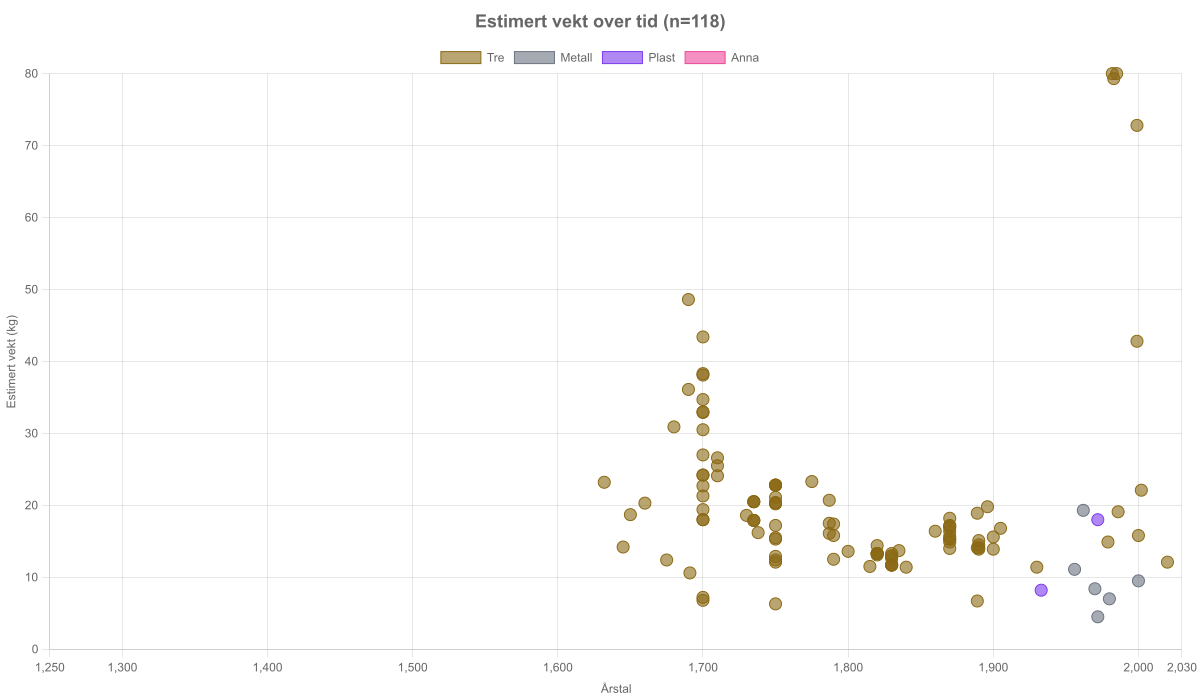
\includegraphics[width=0.8\textwidth]{../charts/01_weight_over_time.png}
    \caption{Utvikling i estimert vekt/volum over tid (basert på 135 norske stolar frå \texttt{stolar.db} og 3D-data).}
    \label{fig:weight}
\end{figure}

\begin{figure}[H]
    \centering
    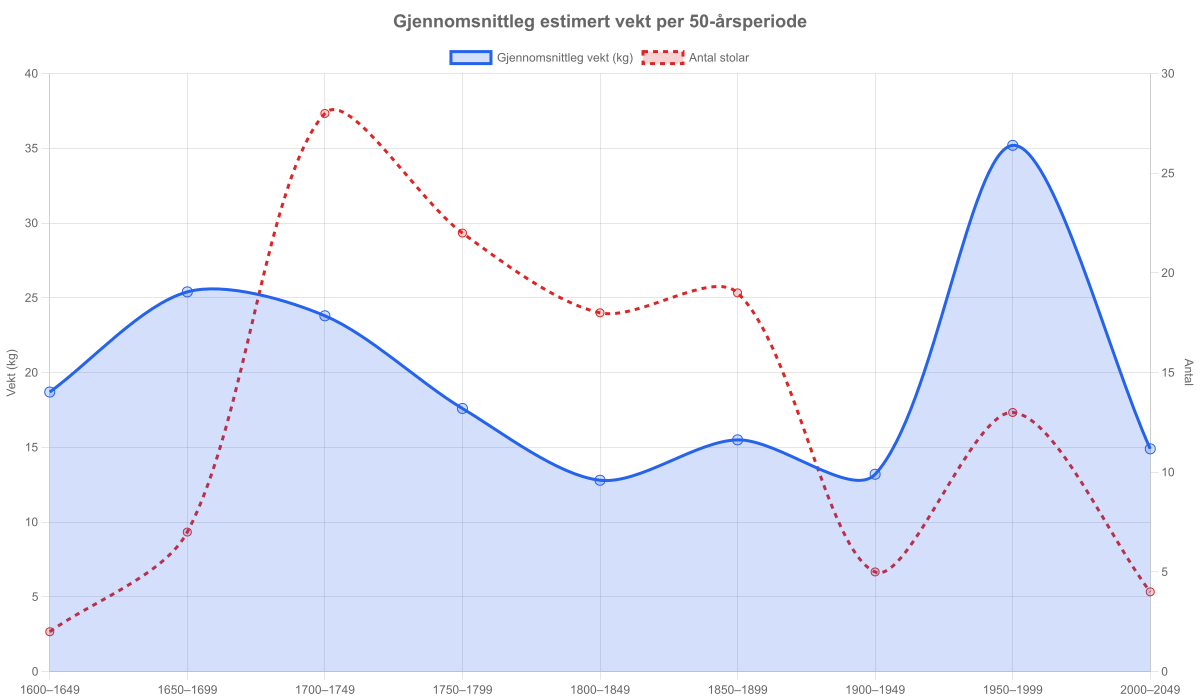
\includegraphics[width=0.8\textwidth]{../charts/03_avg_weight_per_period.png}
    \caption{Gjennomsnittleg vekt per stilepoke. Merk det markante droppet etter den industrielle revolusjonen.}
    \label{fig:avgweight}
\end{figure}

\section{Oppsummering}
Stolsamlinga i Nasjonalmuseet er eit fysisk arkiv over menneska si evne til å forme verda rundt seg. Ved å hente ut kvantitative data frå historiske objekt -- frå den massive furuplanken til den optimaliserte stålstrukturen -- beviser vi at møbelhistoria er ei reise mot auka materiell «fitness». Dette fundamentet peikar fram mot eit skifte i korleis vi kan forstå og undervise i industridesign: Ikkje som rein formgjeving, men som objektiv optimalisering (Jony Ive) forankra i rasjonell konstruksjon (Le Corbusier).

\bibliographystyle{plainnat}
\bibliography{referansar}

\end{document}